{\fontsize{12pt}{22pt} \textbf{DBSCAN}\par}

\vspace{5mm}

DBSCAN (Density-Based Spatial Clustering of Applications with Noise) is an algorithm allowing to find clusters based on a density and classication of points. 

Note: density can be seen as the number of points in one's neighborhood. \\

The algorithm has two main parameters:

$\epsilon$ is the size of the neighborhood.

$MinPts$ is the minimum points in $\epsilon$-neighborhood to define a cluster.  \\

Every point is classified among three categories:

- A \textit{core} point has at least $MinPts$ points in its $\epsilon$-neighborhood.

- A \textit{border} point has less than $MinPts$ points in its neighborhood but at least one core point is present.

- An \textit{outlier} is neither a core nor a border point. \\

\begin{center}
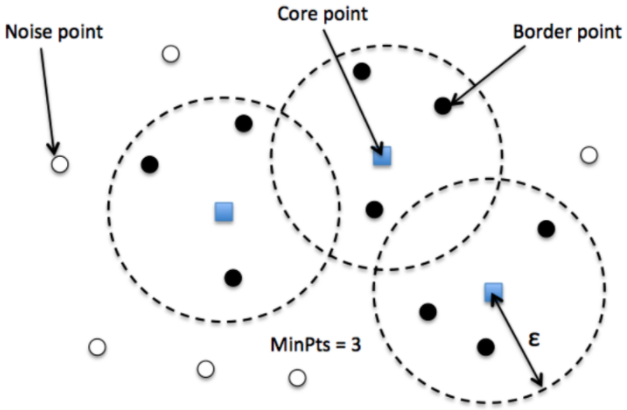
\includegraphics[scale=0.3]{DBSCAN.png}
\end{center}

DBSCAN uses \textit{density-reachability} to navigate through points and identify clusters.

Density-reachability: a point $y$ is \textit{density-reachable} from $x$ if there is a path $p_1,..., p_n$ with $p_1=x$ and $p_n=y$ where each $p_{i+1}$ on the path must be core points with the possible exception of $p_n$. \\

\begin{algorithm}
\caption{DBSCAN (simplified)}
\begin{algorithmic}
\While{some points are unclassified}
\State pick random point
\If{classified \& core point}
\For{$neighbor$ in $density\_reachable\_neighbors$}
\If{outlier}
\State change to border
\EndIf 
\State add to cluster
\EndFor
\Else
\If{core point}
\State label as core point
\Else
\State label as outlier
\EndIf
\EndIf 
\EndWhile
\end{algorithmic}
\end{algorithm}

Its main advantages over k-means is that it can find non convex clusters as well as detecting outliers (noise). \\

\underline{Parameter estimation} \\

High $MinPts$ or low $\epsilon$ means higher density is necessary to form a cluster. \\

The original DBSCAN paper proposes a method to define $\epsilon$. The method consists in plotting the k-th distance to each point in decreasing order. The largest values (left of the graph) are associated with outliers; smaller values are associated with cluster points. The inflection point is the \textbf{cluster point} with the highest k-distance; it corresponds to the epsilon we are looking for.

\begin{center}
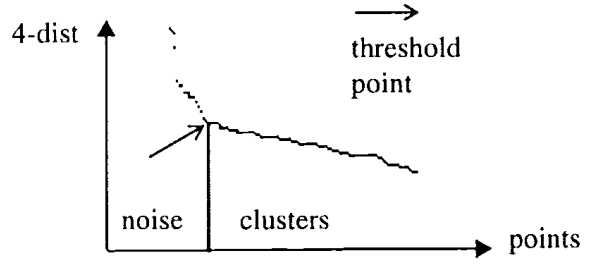
\includegraphics[scale=0.4]{DBSCAN_epsilon.png}
\end{center}

The authors mention that finding the threshold point automatically is rather difficult. They suggest that the user has to estimate the percentage of noise.
I propose the following method to determine the threshold dynamically:

- Compute the slope of the line that links the first and last point in the graph.

- Find the two successive points with the closest slope.

The threshold will be the first of the two found points.

\begin{center}
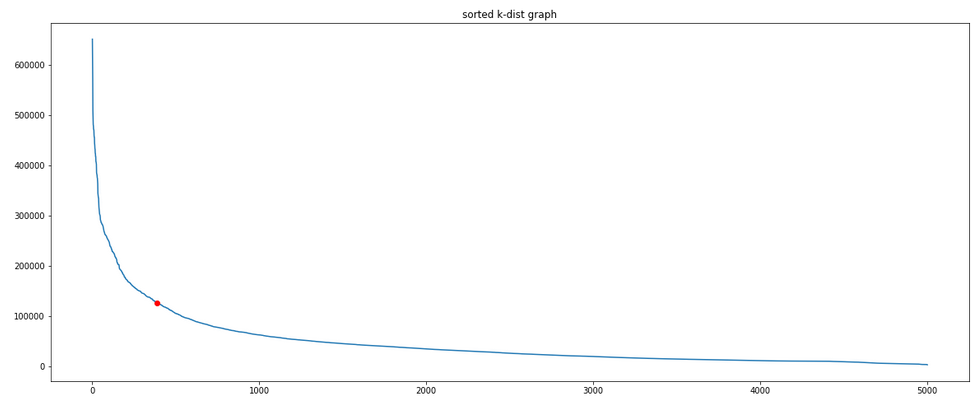
\includegraphics[scale=0.4]{DBSCAN_epsilon_2.png}
\end{center}

\vspace{5mm}